\input{../article_base.tex}
\title{פתרון מטלה 01 --- אנליזה על יריעות, 80426}
\usepackage{pgfplots}
\pgfplotsset{compat=1.18}

\begin{document}
\maketitle
\maketitleprint{}

\question{}
תהי המסילה $\gamma : [0, 2] \to \RR^2$ המוגדרת על־ידי,
\[
	\gamma(t) = (t^2, t^3)
\]

\subquestion{}
נחשב את האורך של $\gamma$.
\begin{solution}
	נבחין כי $\dot{\gamma}(t) = (2t, 3t^2)$ מחישוב ישיר, וכן מהגדרה,
	\[
		l(\gamma)
		= \int_\gamma 1\ dl
		= \int_0^2 \lVert \dot{\gamma}(t) \rVert\ dt
		= \int_0^2 \sqrt{4t^2 + 9t^4}\ dt
		= \int_0^2 t \sqrt{4 + 9t^2}\ dt
	\]
	נשתמש בכלל ההצבה עבור $u = t^2, du = 2t dt$ ונקבל
	\[
		\int_0^2 t \sqrt{4 + 9t^2}\ dt
		= \frac{1}{2} \int_0^4 {(4 + 9u)}^\frac{1}{2}\ dt
		= \left. \frac{1}{2} {(4 + 9u)}^\frac{3}{2} \cdot \frac{1}{9} \cdot \frac{2}{3} \right\rvert_{u = 0}^{u = 2}
		= \frac{1}{3} ({40}^\frac{3}{2} - 4^\frac{3}{2})
	\]
\end{solution}

\subquestion{}
נחשב את הישר המשיק ואת משיק היחידה ל־$\gamma$ ב־$t = 1$.
\begin{solution}
	לפי הגדרת הישר המשיק נחשב ונקבל,
	\[
		l
		= \Sp\{ \dot{\gamma}(1) \}
		= \Sp\{ (2, 3) \}
		= \{ (2, 3)t \mid t \in \RR \}
	\]
	וכן משיק היחידה הוא
	\[
		\vec{T}_\gamma(1)
		= \frac{\dot{\gamma}(1)}{\lVert \dot{\gamma(1)} \rVert}
		= \frac{(2, 3)}{\sqrt{13}}
	\]
\end{solution}

\question{}
עבור המסילות הבאות נצייר ונחשב את האינטגרל המסילתי של $\gamma : [0, 1] \to \RR^n$ עם הפונקציות הנתונות.

\subquestion{}
נגדיר $\gamma(t) = (t^2, t^2 - t)$ ונחשב את $\int_\gamma F\ d\gamma$ עבור $F(x, y) = (x^2 y, y - 3x)$.
\begin{solution}
	עבור הציור נרצה לבצע רפרצטריזציה של $\gamma$ כך ש־$\gamma \circ \mu = (t, f(t))$, נבחין כי עבור $\mu(t) = \sqrt{t}$ נקבל $f(t) = t - \sqrt{t}$ ב־$[0, 1]$ ולכן נוכל לעבור לציור,
	\begin{otherlanguage}{english}
		\begin{center}
			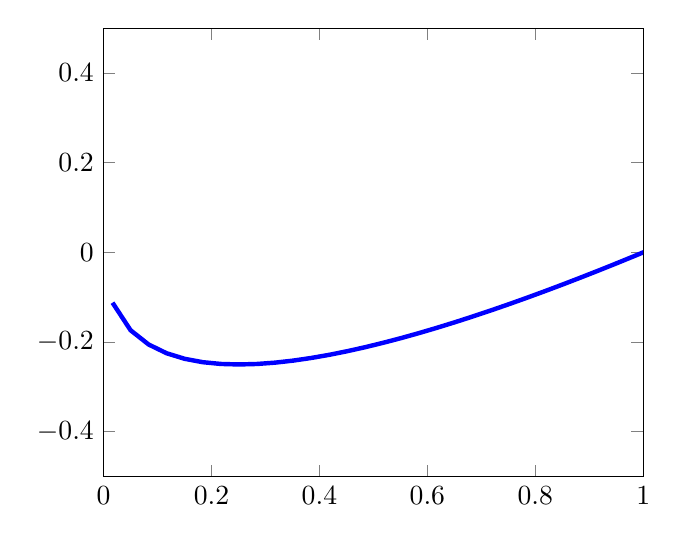
\begin{tikzpicture}
				\begin{axis}[ymin=-0.5,ymax=0.5,xmin=0,xmax=1, samples=300]
					\addplot[blue, ultra thick] (x,{x - sqrt(x)});
				\end{axis}
			\end{tikzpicture}
		\end{center}
	\end{otherlanguage}
	ונעבור לחישוב האינטגרל,
	\begin{align*}
		\int_\gamma F\ d\gamma
		& = \int_0^1 F(\gamma(t)) \cdot \dot{\gamma}(t)\ dt \\
		& = \int_0^1 (t^4 (t^2 - t), t^2 - t - 3t^2) \cdot (2t, 2t - 1)\ dt \\
		& = \int_0^1 2t^5 (t^2 - t) + (2t - 1) (-t - 2t^2)\ dt \\
		& = \int_0^1 2t^7 - 2t^6 - 4t^3 - t\ dt \\
		& = \left. \frac{2}{8} t^8 - \frac{2}{7} t^7 - t^4 - \frac{1}{2} t^2 \right\rvert_{t = 0}^{t = 1} \\
		& = \frac{1}{4} - \frac{2}{7} - 1 - \frac{1}{2} - 0
	\end{align*}
\end{solution}

\subquestion{}
נגדיר $\gamma(t) = (t, \cos t, \sin t)$ וכן $F(x, y, z) = (0, -z, y)$.
\begin{solution}
	נצייר,
	\begin{otherlanguage}{english}
		\begin{center}
			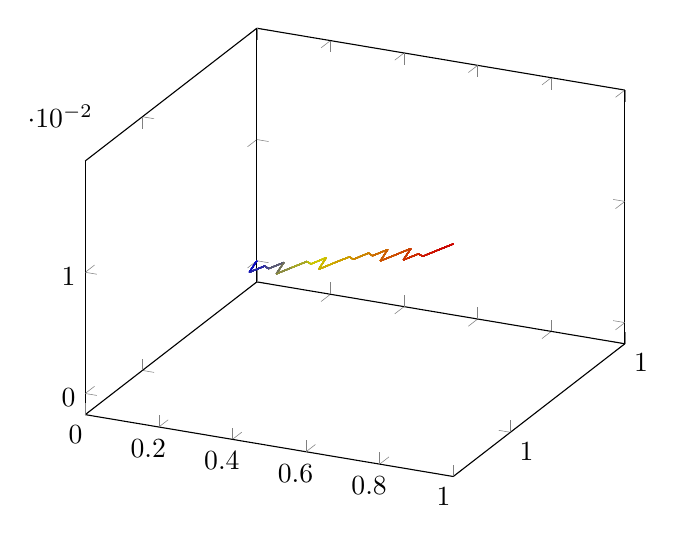
\begin{tikzpicture}
				\begin{axis}
				\addplot3[
					surf,
					domain=0:1,
					] (x,{cos(x)},{sin(x)});
				\end{axis}
			\end{tikzpicture}
		\end{center}
	\end{otherlanguage}
	נעבור לחישוב האינטגרל,
	\[
		\int_\gamma F\ d\gamma
		= \int_0^1 F(\gamma(t)) \cdot \dot{\gamma}(t)\ dt
		= \int_0^1 (0, -\sin t, \cos t) \cdot (1, -\sin t, \cos t)\ dt
		= \int_0^1 \sin^2 t + \cos^2 t\ dt
		= \int_0^1 1\ dt
		= 1
	\]
\end{solution}

\subquestion{}
נגדיר $\gamma(t) = (2t - 1, \sqrt{1 - {(2t - 1)}^2})$, ואת הפונקציה $f(x, y) = x y^4$.
\begin{solution}
	נתחיל בציור,
	\begin{otherlanguage}{english}
		\begin{center}
			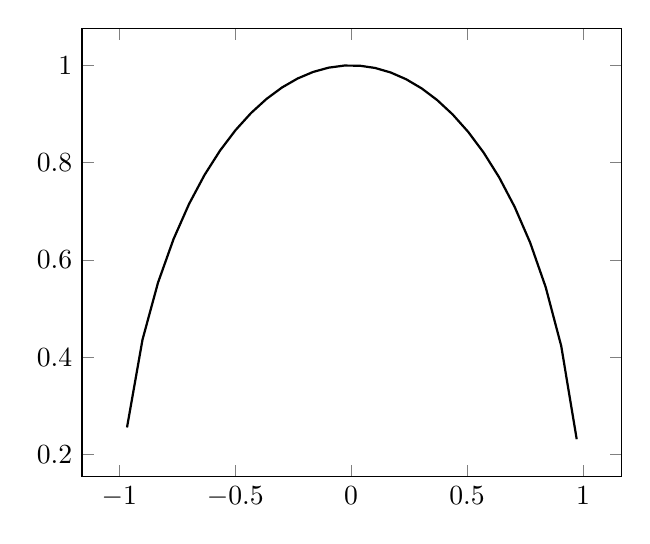
\begin{tikzpicture}
				\begin{axis}[
					%ymin=-0.5,ymax=0.5,
					%xmin=0,xmax=1,
					samples=300
					]
					\addplot[black, thick] ({2 * x - 1},{sqrt(1 - (2 * x - 1)^2)});
				\end{axis}
			\end{tikzpicture}
		\end{center}
	\end{otherlanguage}
	ונעבור לחישוב האינטגרל.
	נבצע רפרמטריזציה יחד עם $\mu : [-1, 1] \to [0, 1]$ על־ידי $\mu(t) = \frac{t + 1}{2}$ ונקבל $(\gamma \circ \mu)(t) = (t, \sqrt{1 - t^2})$,
	ולאחר מכן נקבל $\bar{\gamma} : [0, \pi] \to \RR^2$ המוגדרת על־ידי $\bar{\gamma}(t) = (\cos t, \sin t)$.
	בנוסף גם $\dot{\bar{\gamma}}(t) = (-\sin t, \cos t)$ וכן $f(\bar{\gamma}(t)) = \cos(t) \sin^4(t)$, לכן
	\[
		\int_{\bar{\gamma}} f\ ds
		= \int_0^\pi \cos(t) \sin^4(t) \sqrt{\sin^2(t) + \cos^2(t)}\ dt
		= \left. \frac{1}{5} \sin^5(t) \right\rvert_{t = 0}^{t = \pi}
		= 0
	\]
\end{solution}

\question{}
תהי מסילה רגולרית $\gamma : [a, b] \to U$ ותהי $\bar{\gamma}$ המסילה נורמלית שלה. \\
נוכיח שכמות האורך המכוסה על־ידי $\bar{\gamma}$ בכל קטע היא האורך של הקטע, כלומר לכל $s_1 < s_2 \in [0, l(\gamma)]$ מתקיים $l(\bar{\gamma} \mid_{[s_1, s_2]}) = s_2 - s_1$.
\begin{proof}
	
\end{proof}

\end{document}
